% numerical.tex

\cleardoublepage
\chapter{Optimised Trajectory Including Fly-Back}\label{chapter:Flyback}

This chapter presents the optimised trajectory of the launch system, including the fly-back of the SPARTAN. The combined optimisation for the ascent/fly-back and third stage trajectory is currently operational in LODESTAR. Figures \ref{fig:ascent}-\ref{fig:groundtrack} show an example of a combined optimised trajectory for the ascent/return of the SPARTAN and the ascent of the third stage, for maximum payload-to-orbit. However, the aerodynamic and propulsive databases are currently being updated, and will change the optimised results slightly. It is not expected that the major points of interest in the trajectory will change.



 The ascent trajectory will be compared to the optimised ascent without fly-back calculated in Section \ref{chapter:Ascent}. The SPARTAN compensates for the fly-back by banking during ascent. This requires additional angle of attack, and results in less velocity and a smaller pull-up. A small deviation from 50kPa dynamic pressure is observed directly before pull-up, accompanied by a rise in bank angle. This manoeuvre reduces the total range during ascent for minimal velocity losses, decreasing the fuel necessary for the return flight. 
 

The return flight analysis consists of a modified form of the paper 'Fly-Back of a Scramjet-Powered Accelerator', presented at Scitech 2018. Currently, this analysis is for a standalone optimised fly-back from a fixed point.  The results will modified to be for the fly-back portion of the combined optimisation. The analysis in this section is expected to change little. 



The sensitivity analysis in this chapter will be expanded, and will be compared against the sensitivity analysis without fly-back, presented in Chapter \ref{chapter:Ascent}, to determine how the fly-back changes the sensitivity of the trajectory to the design parameters of the SPARTAN. As in Chapter \ref{chapter:Ascent}, the validation of each case will be discussed, with forward simulation comparisons and optimality condition validations provided in appendices. 




\section{Combined SPARTAN Ascent-Descent \& Third Stage Example}

This section contains a current example of a concurrently optimised SPARTAN ascent/fly-back and third stage ascent. 

\begin{figure}[H]
	\centering
	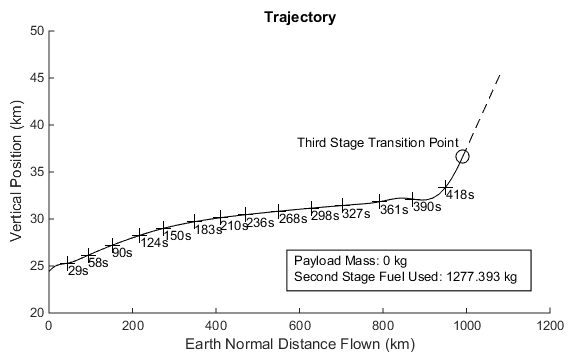
\includegraphics[width=0.9\linewidth]{figures/7_Full/Ascent}
	\caption{The flight path of the SPARTAN ascent.}
	\label{fig:ascent}
\end{figure}
\begin{figure}[H]
	\centering
	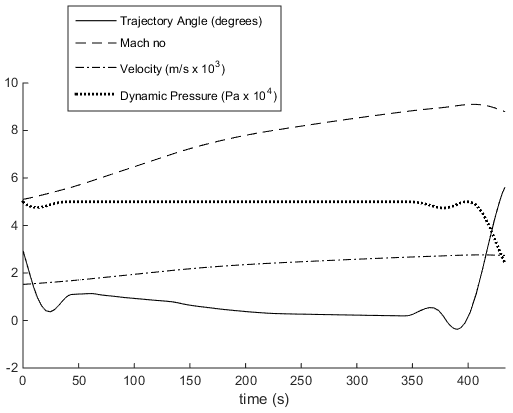
\includegraphics[width=0.7\linewidth]{figures/7_Full/Ascent-Aero}
	\caption{Aerodynamic parameters of the SPARTAN ascent.}
	\label{fig:ascent-aero}
\end{figure}
\begin{figure}[H]
	\centering
	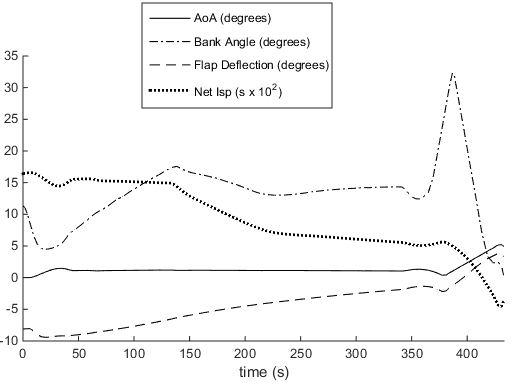
\includegraphics[width=0.7\linewidth]{figures/7_Full/Ascent-Vehicle}
	\caption{Vehicle parameters of the SPARTAN ascent.}
	\label{fig:ascent-vehicle}
\end{figure}
\begin{figure}[H]
	\centering
	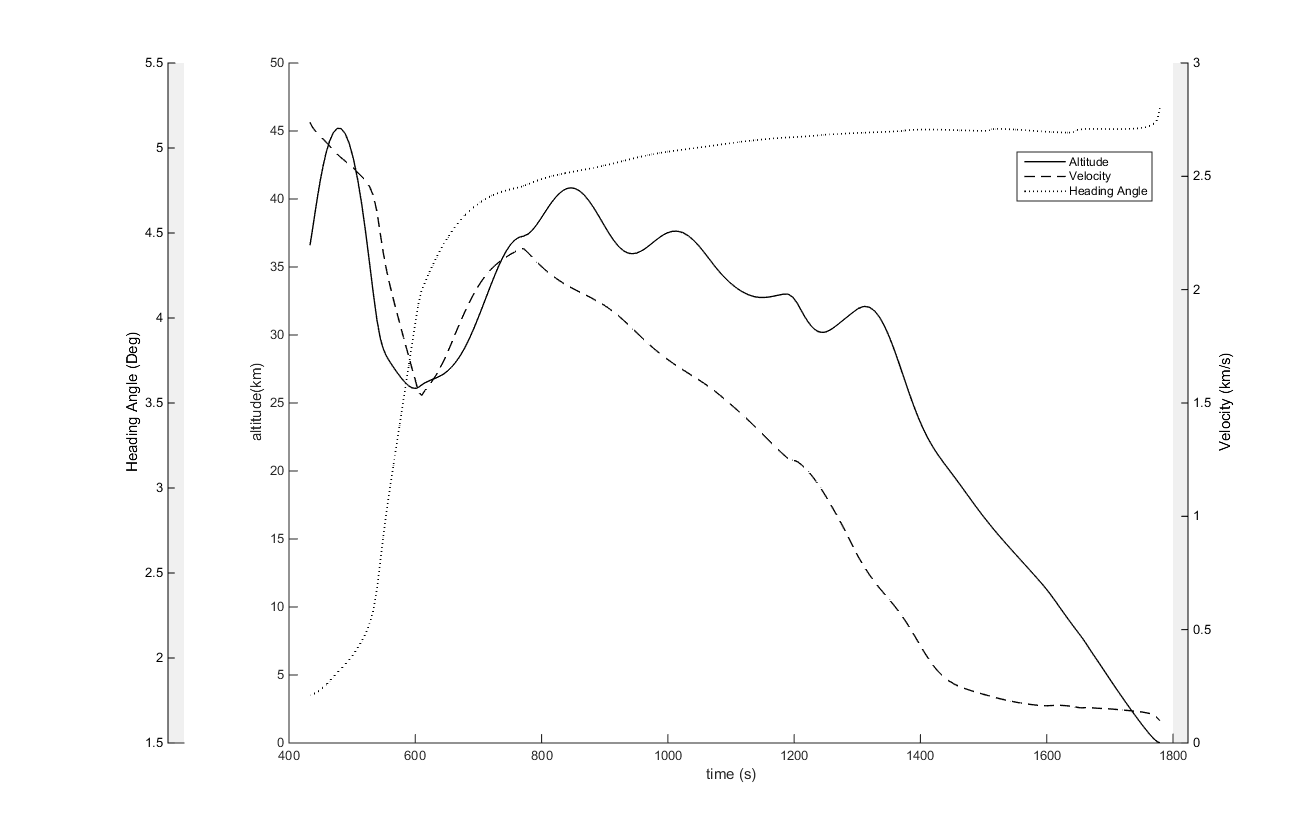
\includegraphics[width=0.7\linewidth]{figures/7_Full/FlyBack1}
	\caption{The flight path of the SPARTAN fly-back.}
	\label{fig:flyback1}
\end{figure}
\begin{figure}[H]
	\centering
	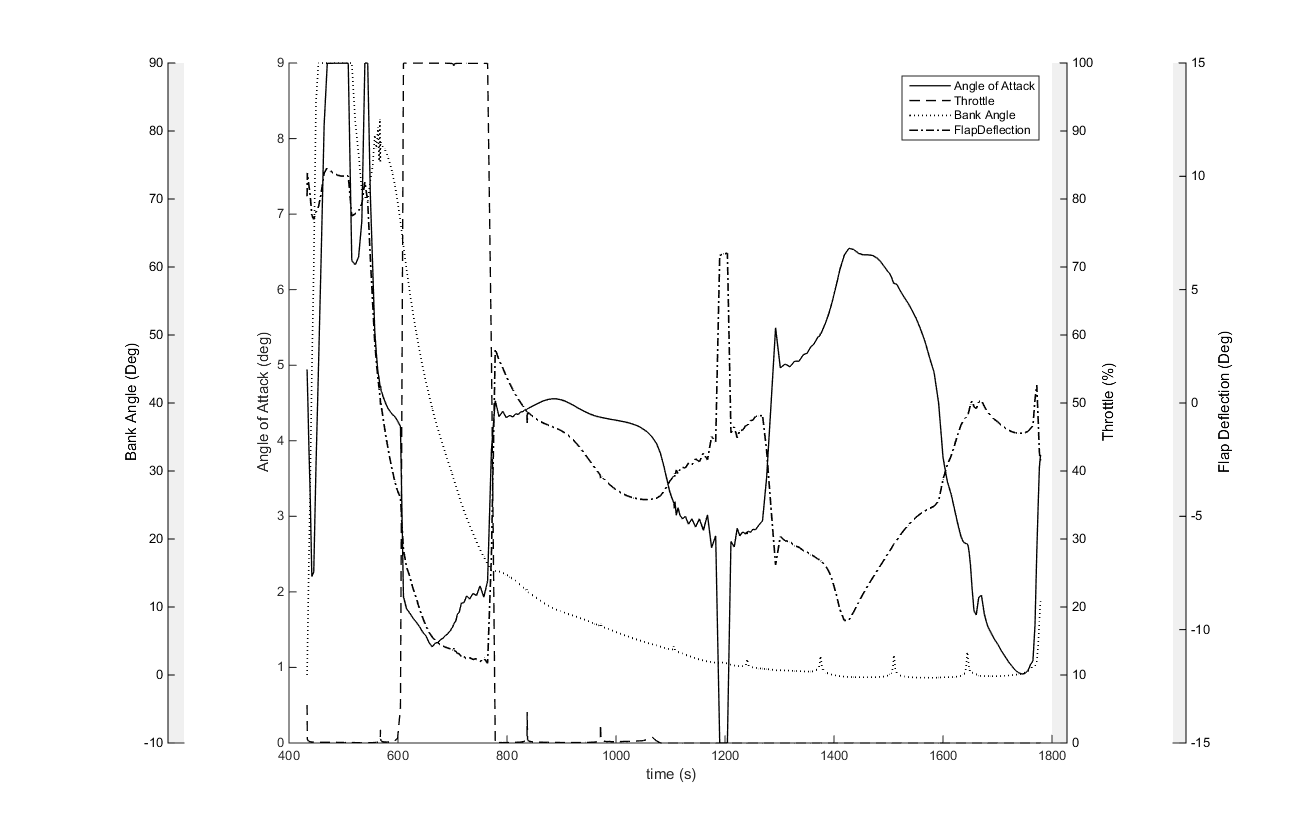
\includegraphics[width=0.7\linewidth]{figures/7_Full/FlyBack2}
	\caption{Vehicle parameters of the SPARTAN fly-back.}
	\label{fig:flyback2}
\end{figure}
\begin{figure}[H]
	\centering
	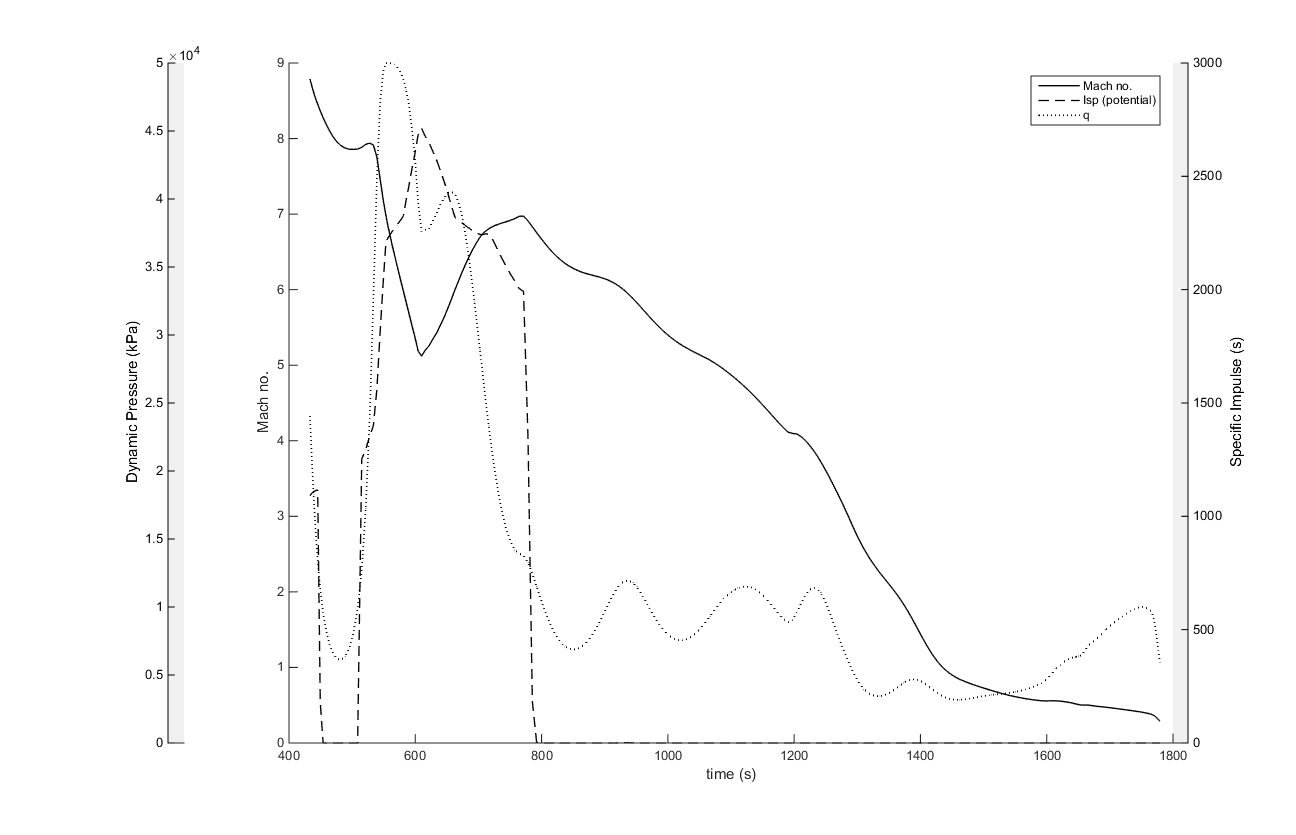
\includegraphics[width=0.7\linewidth]{figures/7_Full/FlyBack3}
	\caption{Aerodynamic and propulsion parameters of the SPARTAN fly-back.}
	\label{fig:flyback3}
\end{figure}
\begin{figure}[H]
	\centering
	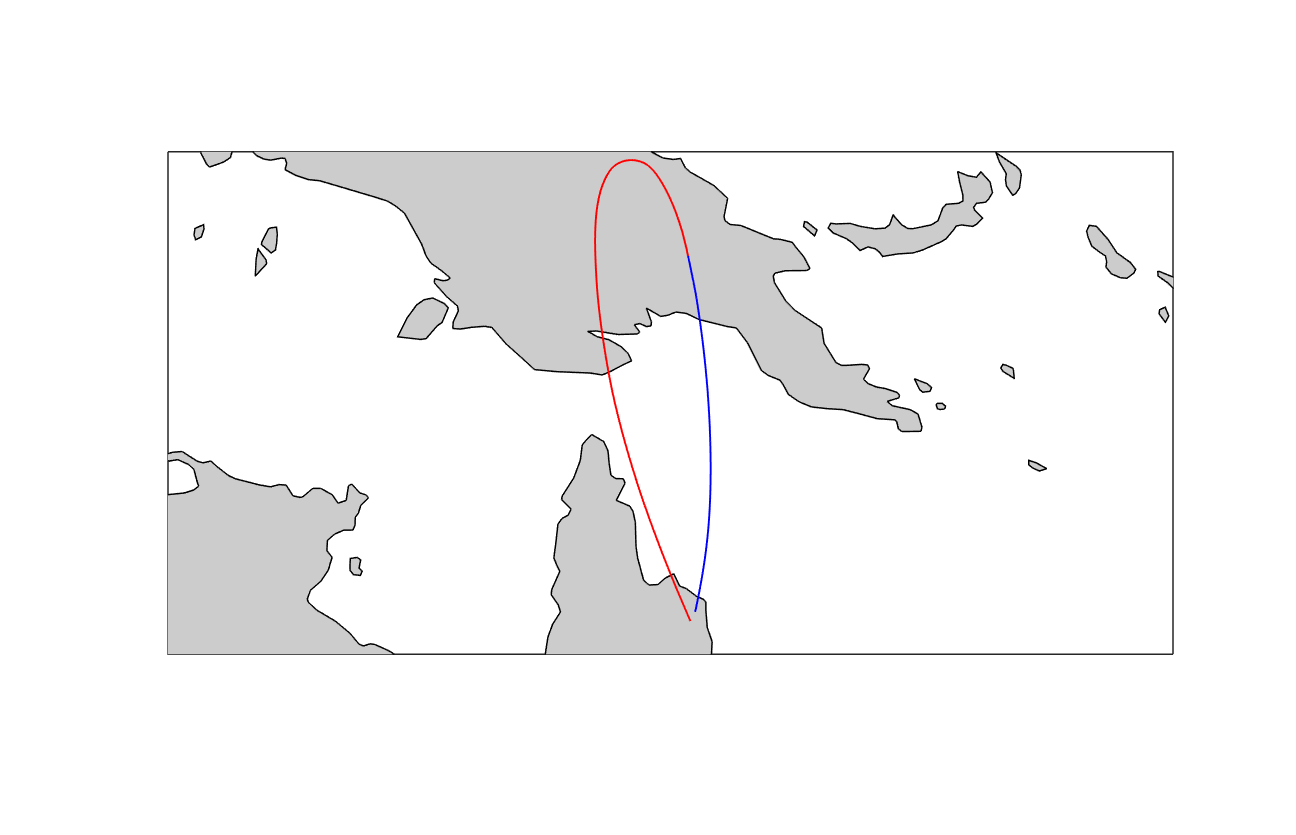
\includegraphics[width=0.7\linewidth]{figures/7_Full/groundtrack}
	\caption{The ground track of the ascent and fly-back of the SPARTAN.}
	\label{fig:groundtrack}
\end{figure}



\section{Fly-Back Trajectory Analysis}
The fly-back of the SPARTAN is optimised using LODESTAR. The fly-back is optimised for minimum fuel usage, with initial conditions constrained to be similar to the intended third stage release point, and end position constrained within 12.7km of the initial launch site, at  15.3$^\circ$S,144.9$^\circ$E\cite{ForbesSpyratos2018}. The margin of 12.7km is allowed so as to not over-constrain the end position within LODESTAR, and it is assumed that the landing strip will not be at the exact location of the launch site. The angle of attack is limited to 10$^\circ$, to ensure vehicle stability. The bank angle is limited to 90$^\circ$ to produce a conservative solution and to limit any possible design complications that may arise from inverted flight. The dynamic pressure is limited to 50kPa, the structural limit of the vehicle. The scramjet engines are limited to only operate above 20kPa dynamic pressure, an estimated lower limit on the operable mass flow rate.
The end of the trajectory is constrained to sub-200m altitude, and a trajectory angle range between -10$^\circ$ and 0$^\circ$ to ensure that the SPARTAN can perform a landing manoeuvre. These constraints ensure that the vehicle is approaching the landing site at the end of the optimised trajectory. The end velocity is only limited to be greater than 0m/s. It can be assumed that the optimal fly-back trajectory minimises end velocity as shown in the optimised trajectory results. 
It is also assumed that the vehicle is able to carry any necessary fuel in addition to the fuel required during the ascent trajectory, allowing the initial conditions to be kept constant. The potential specific impulse is shown along the trajectory, this is the specific impulse obtainable from the C-REST engines should they be powered on.

\subsection{Optimised Trajectory}
\begin{figure}[t]
	\centering
	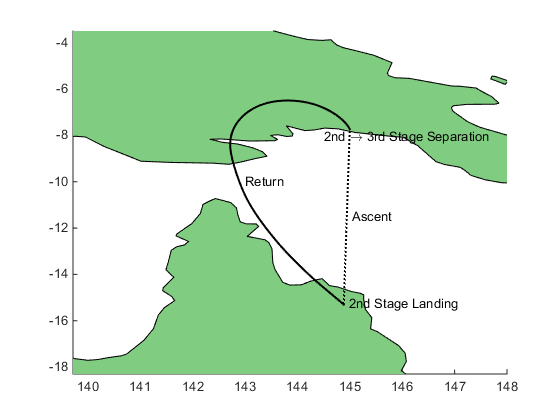
\includegraphics[width=0.6\linewidth]{Figures/6_flyback/lon-lat}
	\vspace{-10pt}
	\caption{ Ground track of the optimised fly-back of the SPARTAN vehicle.}
	\label{fig:lon-lat}
\end{figure}  


%\begin{figure}[h]
%	\centering
%	\includegraphics[width=0.9\linewidth]{Figures/Traj1}
%	\vspace{-10pt}
%	\caption{Trajectory data for the fly-back of the SPARTAN vehicle. Optimised for minimum fuel usage using LODESTAR. }
%	\label{fig:Traj1}
%\end{figure}
%\begin{figure}[h]
%	\centering
%	\includegraphics[width=0.9\linewidth]{Figures/Traj2}
%	\vspace{-10pt}
%	\caption{Aerodynamic and performance data for the optimised fly-back of the SPARTAN vehicle. }
%	\label{fig:Traj2}
%\end{figure}
%\begin{figure}[h]
%	\centering
%	\includegraphics[width=0.9\linewidth]{Figures/Traj3}
%	\vspace{-10pt}
%	\caption{Control data for the optimised fly-back of the SPARTAN vehicle.}
%	\label{fig:Traj3}
%\end{figure}

\begin{figure}
	\begin{subfigure}[b]{\textwidth}
		\includegraphics[width=\linewidth]{Figures/6_flyback/Traj1}
		\vspace{-15pt}
		\caption{ Flight path.}
		\label{fig:Traj1}
	\end{subfigure}
	
	\begin{subfigure}[b]{\textwidth}
		\includegraphics[width=\linewidth]{Figures/6_flyback/Traj2}
		\vspace{-15pt}
		\caption{Aerodynamic and performance data. }
		\label{fig:Traj2}
	\end{subfigure}
	
	\begin{subfigure}[b]{\textwidth}
		\includegraphics[width=\linewidth]{Figures/6_flyback/Traj3}
		\vspace{-15pt}
		\caption{Control time histories.}
		\label{fig:Traj3}
	\end{subfigure}
	\caption{Trajectory data for the fly-back of the SPARTAN vehicle. Optimised for minimum fuel usage using LODESTAR.}
	\label{fig:AllTraj}
\end{figure}

The optimised fly-back trajectory is shown in Figures \ref{fig:lon-lat} and \ref{fig:AllTraj}.
The fly-back is initiated from the optimised second-third stage separation point at 7.7$^\circ$S,145.0$^\circ$E, 34.5km altitude, 2.9$^\circ$ trajectory angle, 2881m/s velocity and 102$^\circ$ heading angle, corresponding to the conditions of optimal third stage release described in Section \ref*{sec:opt}. 
The SPARTAN is shown to be capable of fly-back, using 166.0kg of fuel, a total increase in the fuel usage of the SPARTAN of 10.6\%.
The optimised trajectory has four distinct parts; 1. initial turn, 2. boost phase, 3. hop-glide, and 4. approach. 

\subsubsection{ Initial Turn}
The SPARTAN starts at the maximum bank angle of 90$^\circ$, and sustains this bank angle for 34.4s. At this point, the altitude of the SPARTAN decreases, and the vehicle is close to hitting the dynamic pressure of 50kPa. To avoid exceeding this limit, the bank angle is reduced to 71.2$^\circ$, allowing the vehicle to generate sufficient lift to slow its descent. The bank angle in then increased again, to 80.7$^\circ$ at 70.8s. After this time, the bank angle is gradually reduced. 

\subsubsection{ Boost Phase}
Soon after the bank angle begins to reduce, at 118.7s flight time and Mach 5.71, the scramjet engines are ignited. The C-REST engines are powered-on at a point of high potential specific impulse, at a low Mach number, and burn for 119.8s. The altitude of the SPARTAN is raised during the majority of the burn, ensuring that the Mach number is kept low for maximum efficiency\cite{Preller2017}, as shown in Figure \ref{fig:AllTraj}. The maximum altitude is limited by the lower dynamic pressure limit of the C-REST engines of 20kPa. The bank angle of the vehicle is reduced to produce increased lift, so as to increase the altitude of the SPARTAN, while also maximising the specific impulse of the scramjet engines by keeping the angle of attack low. Low angle of attack decreases the temperature and raises the Mach number, at the inlet of the C-REST engines. While these effects partially offset each other\cite{Preller2017}, the temperature increase is more significant, and decreasing angle of attack has the net effect of increasing the specific impulse of the C-REST engines. This increase in specific impulse is balanced by a decrease in the L/D of the SPARTAN at angle of attack values lower than 4$^\circ$, as illustrated in Figure \ref{fig:LD}. However, the specific impulse has a more significant impact than L/D during this phase, resulting in the optimised angle of attack being kept low. At 204s the angle of attack is increased, bringing the L/D of the vehicle towards maximum and initiating the first 'skip' of the skip-glide phase.  


\subsubsection{ Skip-Glide}
During the unpowered trajectory after the burn phase, the angle of attack is controlled so that the L/D of the SPARTAN is close to the maximum. Initially, the SPARTAN performs several 'skips' after the scramjet burn. These are due to the high L/D of the SPARTAN above Mach 4, and are aided by the angle of attack, which is controlled to emphasize the size of the skips. These skips are consistent with research which has shown that a periodic skipping trajectory increases the downrange distance achievable by hypersonic vehicles\cite{Eggers1957,Kanda2007}. 


\subsubsection{ Approach}
After the skip phase, as the vehicle is approaching Mach 1, the angle of attack is reduced gradually to bring the SPARTAN down to 200m altitude, in a controlled manner. 
At the end of the trajectory the SPARTAN levels out, and reaches 200m altitude at -9.6$^\circ$ trajectory angle and 119.8m/s velocity. These conditions are similar to those of the space shuttle at landing\cite{Ryba2017}, and it is assumed that the SPARTAN is able to perform a landing manoeuvre after this point. 








\subsection{Sensitivity Analysis}
To investigate the robustness of the fly-back trajectory to vehicle design; the drag coefficient and specific impulse of the SPARTAN are varied by $\pm 10\%$, and the new optimal fly-back trajectories are calculated using LODESTAR. These optimised trajectories, shown in Figures \ref{fig:CdVariation} and \ref{fig:IspVariation}, investigate the effects of potential performance variation caused by changes in the vehicle design.
The consistency of the trajectory shape indicates that the optimal solution is robust with variation in the aerodynamic parameters and specific impulse of the SPARTAN. The optimised trajectories show clear trends with variation in vehicle parameters.

Increasing the drag coefficient causes the fuel necessary for fly-back to increase by +51.5kg (+31.0\%). Conversely, decreasing the drag coefficient by 10\% causes the fuel necessary for  fly-back to decrease by -58.0kg (-34.9\%). 
When the drag is increased (ie. L/D is decreased), the scramjet engine burn phase begins earlier, and continues for longer. 
The greater burn time allows the maximum altitude attained during the initial 'skip' to be higher. 
This additional altitude is necessary as the greater drag causes the velocity, and consequentially altitude, of the SPARTAN to decrease more rapidly.


Increasing the specific impulse causes the fuel necessary for fly-back to decrease by -11.5kg (-6.9\%), while decreasing the specific impulse causes the fuel necessary to rise by +22.9kg (+13.8\%). The start of scramjet burn is consistent across different specific impulse test cases. Due to the increase in thrust, the SPARTAN accelerates more rapidly for the higher specific impulse case. As a consequence, the initial 'skip' is performed sooner, and subsequent skips are larger. 

These results indicate that the aerodynamic performance of the SPARTAN has significantly more impact than the efficiency of the scramjet engines on the optimised fly-back trajectory. During the fly-back trajectory, the specific impulse is effecting performance only whilst the scramjet engines are operating, compared with the aerodynamics of the vehicle, which effect performance throughout the trajectory. This suggests that, for maximum fly-back performance, the aerodynamic performance should be given preference over engine efficiency in the design of fly-back hypersonic accelerators. 

\begin{figure}[ht]
	\centering
	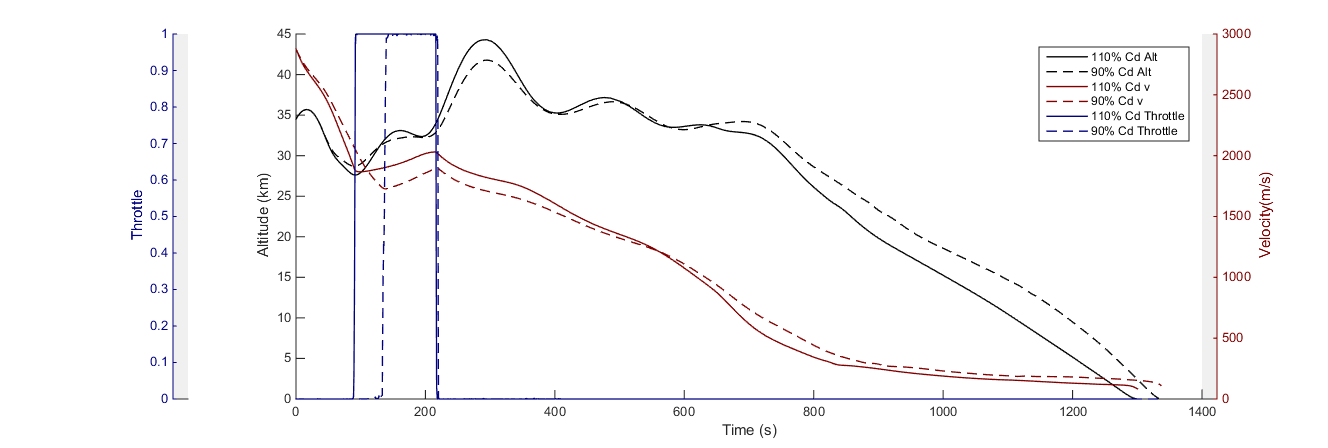
\includegraphics[width=0.9\linewidth]{Figures/6_flyback/CdVariation}
	\caption{Comparison of optimal trajectories with $\pm10\%$ $C_D$ variance.}
	\label{fig:CdVariation}
\end{figure}

\begin{figure}[ht]
	\centering
	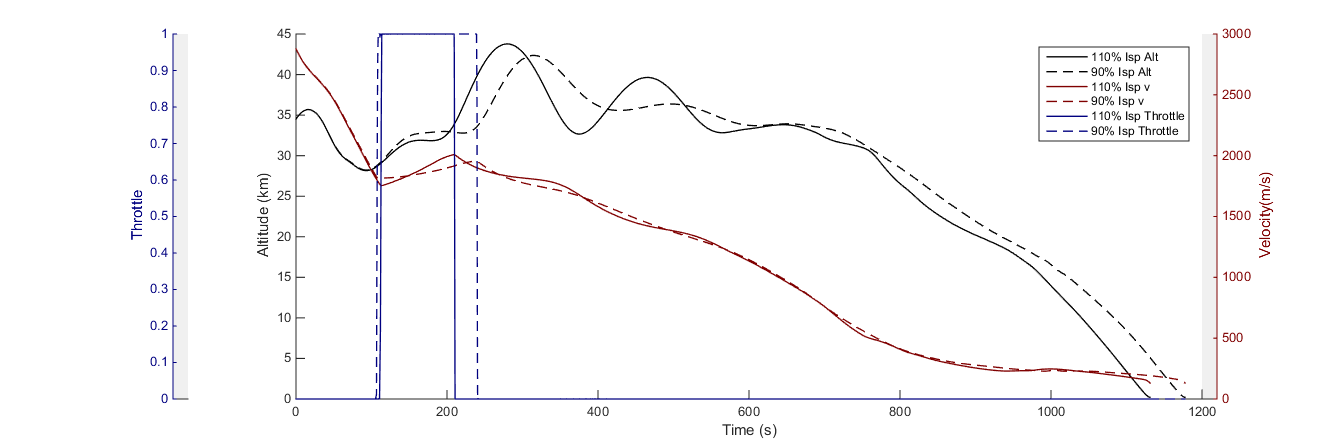
\includegraphics[width=0.9\linewidth]{Figures/6_flyback/IspVariation}
	\caption{Comparison of optimal trajectories with $\pm10\%$ $I_{SP}$ variance.}
	\label{fig:IspVariation}
\end{figure}



\subsection{Conclusion}
The fly-back trajectory of the SPARTAN hypersonic vehicle is investigated, from separation at 7.7$^\circ$S,145.0$^\circ$E to landing at 15.3$^\circ$S,144.9$^\circ$E, corresponding to a near 180$^\circ$ turn and a fly-back of 878km. The aerodynamics of the SPARTAN are calculated using CART3D, an inviscid CFD package, over the range of Mach numbers and angle of attack values of flight. The optimal trajectory of the SPARTAN is calculated, to fly-back to the initial launch position with minimum fuel. The optimal trajectory is calculated using the launch vehicle optimal control program LODESTAR. It is found that the SPARTAN is capable of returning to its initial launch position, using 166.0kg of fuel. The optimal trajectory terminates when SPARTAN reaches 200m altitude at a velocity of 119.8m/s. After this point, it is assumed that the SPARTAN lands on a traditional runway, at similar conditions to the space shuttle.  
This result indicates that the fly-back of a hypersonic launch vehicle from high velocity separation at a Mach number greater than nine, returning to its initial launch site using scramjet hypersonic airbreathing engines, is feasible. This fly-back to the the original launch site is a crucial component for low cost access-to-space using scramjets. 

The coefficient of drag of the SPARTAN and specific impulse of the scramjet engines were independently varied by $\pm10\%$ and the new optimal trajectories calculated to assess the robustness of the fly-back trajectory to uncertainties in vehicle aerodynamics and scramjet performance. It was found that a $\pm10\%$ variation in $C_D$ results in a +31.0\% or -34.9\% variation in fuel mass burned during fly-back, while a $\pm10\%$ variation in $I_{SP}$ results in a much smaller variation of -6.9\% or +13.8\%. These results indicate that the aerodynamics of a fly-back hypersonic accelerator are much more significant to the fly-back fuel usage than the performance of the scramjet engine. 

